\documentclass[rnd]{mas_proposal}
\usepackage[utf8]{inputenc}
\usepackage{amsmath}
\usepackage{amsfonts}
\usepackage{amssymb}
\usepackage{graphicx}
\usepackage{subcaption}
\usepackage{hyperref}
\usepackage{pdfpages}




\title{Semantic Segmentation of aerial images of forest scenery}
\author{Malika Navaratna, Urvashi Negi, Zain Ul Haq, Simon Deussen}
\supervisors{Prof. Sebastian Houben}
\date{February 2022(WS 2021)}


\begin{document}

\maketitle

\pagestyle{plain}
\tableofcontents
\clearpage
\section{Introduction}
Loss of forest area in Germany is taking place at a high rate and due to factors like lack of rainfall, the spruce bark beetle is infesting and destroying forests in Germany. 
To overcome this and to achieve reforestation at a large scale, measures must be taken that can be completed quickly and automatically which would be faster than doing it manually. 
Nowadays, unmanned Aerial Vehicles (UAVs) or drones are common in various applications such as aerial photography, agriculture, surveillance, product deliveries. UAVs can capture images
by which users can generate high resolution images.  

The above problem of loss of forest cover at a large scale has been identified and a project is in progress by a team at our university. The project is named Garrulus and 
details can be found on their website \cite{hbrs-garrulus}. Garrulus is a project with the aim to reforest damaged forest area using UAVs. The prototype of the UAV would be surveying the 
terrain and would identify areas that are suitable for planting. 
Deep Learning is a field used for terrain surveillance and can provide relevant information. Image segmentation is a subpart of deep learning and is used to label the pixels 
of an image into different classes. Using image segmentation on aerial images captured by the drone is an approach to understand the terrain and plan the suitable land for reforestation.


\subsection{Problem Formulation}

Rapidly changing environment is mainly related due to the deforestation of the land due to various purposes by the humans. Global warming and effected bio-diversity are two major prominent 
effects of deforestation problems but, there are others as well such as desertification, flooding, soil erosion, increased greenhouse gases, and fewer crops etc \cite{Effectso52:online}. 
In order to restore the environment forestation of the land is very important. Autonomous seeding of the deforested land has appeared to be a potential solution for effective forestation of available land. 
 Seeding requires specific land with certain specific conditions to be successful. UAVs can be a potential solution for autonomously seeding the land for effective forestation. 
It is important for autonomous seeding agents such as UAVs to autonomously detect the potential spots for seeding with high rates of success. The main underlying problem is that how a UAV 
find a potential spot for seeding. A UAV collect aerial view of the terrain throughout the flight so there should be a way for a UAV to distinguish a potential spot within a generic aerial 
scenery of the area. A major problem can be locating and identify area of interest in aerial images under different conditions such as uneven illumination, low levels of contrast, or partially 
restricted visibility of the potential land in images. Aerial images of forest are very dense and there are marginal apparent differences between forest and available land due to 
other greenery in the environment, so it becomes a difficult problem to distinguish among a different part of forest i.e., forest and available land as shown in figure \ref{fig:forest-easy} and \ref{fig:forest-hard}.


\begin{figure}
        \centering
        \begin{subfigure}{.5\textwidth}
          \centering
          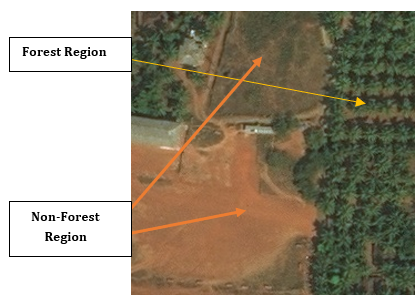
\includegraphics[width=1.0\linewidth]{images/fig1.PNG}
          \caption{Easily distinguishable regions}
          \label{fig:forest-easy}
        \end{subfigure}%
        \begin{subfigure}{.5\textwidth}
          \centering
          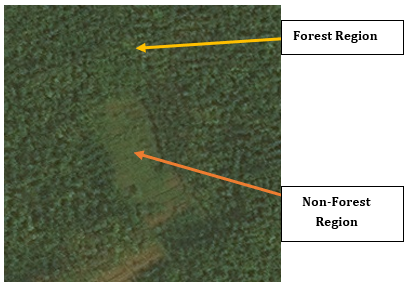
\includegraphics[width=1.03\linewidth]{images/fig2}
          \caption{Not easily distinguishable regions}
          \label{fig:forest-hard}
        \end{subfigure}
        \caption{Sample data}
        \label{fig:Sample data}
\end{figure}


% \begin{figure}[htp] 
%         \centering
%         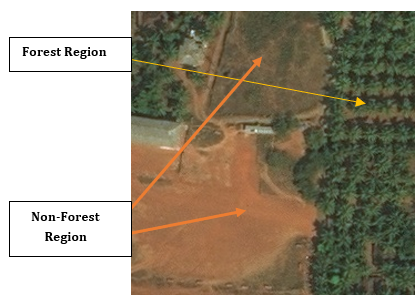
\includegraphics[width=0.5\textwidth]{images/fig1.PNG}
%         \caption{Sample Image with Easily distinguishable regions}%
%         \label{fig:forest-easy}%
% \end{figure}

% \begin{figure}[htp] 
%         \centering
%         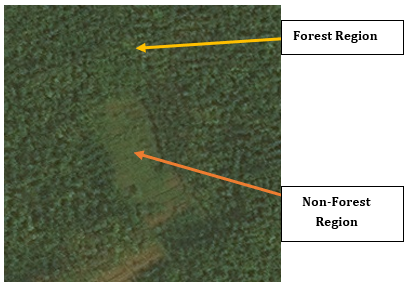
\includegraphics[width=0.5\textwidth]{images/fig2}
%         \caption{Sample Image with difficult distinguishable regions}%
%         \label{fig:forest-hard}%
% \end{figure}



\subsection{Semantic Segmentation}
Semantic segmentation refers to labelling each pixel of an image to a particular class. The figure \ref{fig:semantic_segmentation}  shows an example of a 2D image being classified into classes. In order to distinguish between forest and non forest area, semantic segmentation can be used to classify aerial images and decide the suitable area for reforestation. Architectures such as Fully Convolutional Neural Networks, U-Net are used for semantic segmentation.
% \subfloat{{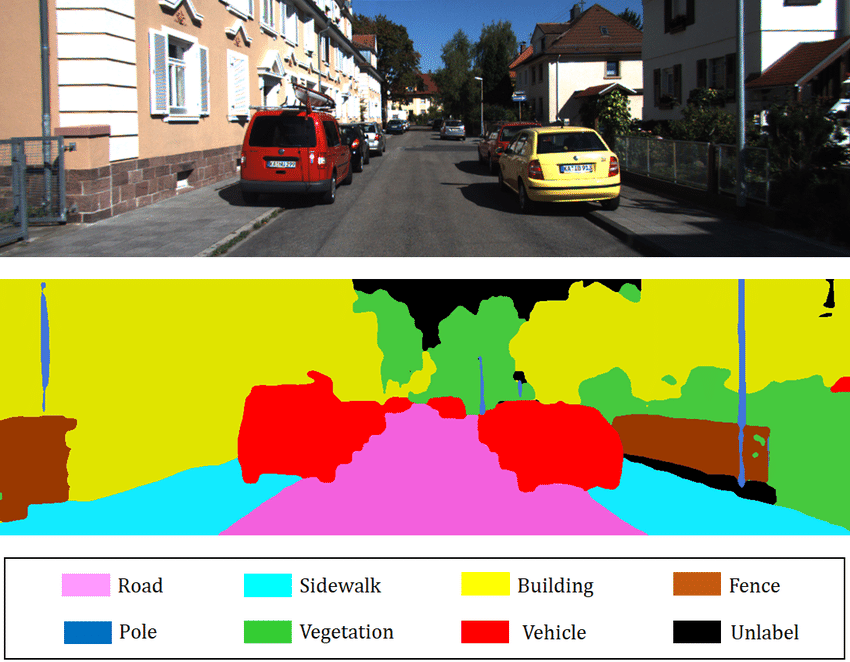
\includegraphics[width=.7\linewidth ]{images/semantic_segmentation.png} }}%

\begin{figure}[htp] 
        \centering
        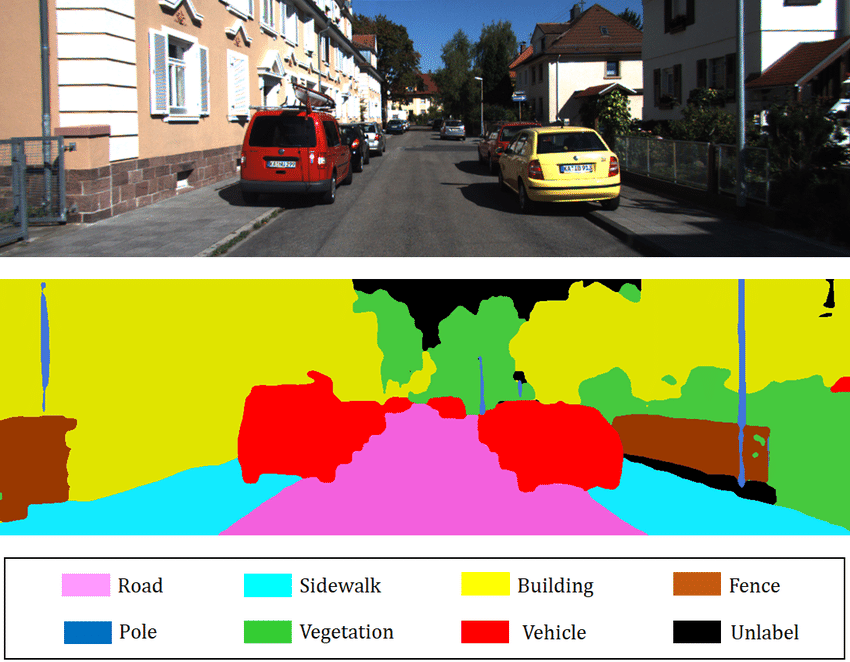
\includegraphics[width=0.65\textwidth]{images/semantic_segmentation.png}
    \caption{Semantic Segmentation as shown in \cite{semantic-segmentation}}%
    \label{fig:semantic_segmentation}%
\end{figure}
\newpage



\section{Related Work}
\subsection{Convolutional Neural Networks}
Convolutional Neural Networks (CNNs) are deep learning architectures that use layers to implement convolutions on the images in order to extract relevant features. They consist of convolutional layer, pooling layer and a fully connected layer. The first breakthrough using CNNs was the AlexNet architecture \cite{alex-net} for the ImageNet challenge. 

The architecture that further improved on this was the VGG architecture that made use of deeper layers than AlexNet in order to get better results. \cite{VGG}. The most well known architectures are the VGG-16 and VGG-19. The performance was further improved by Inception \cite{Inception}. The inceptioon architecture went deeper and each layer had different convolutions to extract different features which were passed on the next layer with the help of a filter. But going deeper was only successful till a certain point and the performance was saturated. But the performance was improved by ResNet \cite{Res-Net} where the authors did not go deeper but instead used skip connections in order to retain the "identity" or the relevant features. 




\subsection{Fully Convolutional Network}
CNNs were designed for recognition of images and assigning a label to the image. Using the convolutional neural network for semantic segmentation was a bottleneck at the fully connected layer because this layer mixes the information from the entire image while getting the output. Therefore the convolutional neural network was modified for the application of semantic segmentation and called Fully Convolutional Network (FCN).\cite{FCN-long} In this architecture, there is a downsampling path that extracts the relevant features, and an upsampling path which helps in localisation. Instead of the fully connected layer, there is a set of 1x1 kernel convolutions. FCNs employ skip connections to retain the information that was lost in the downsampling path. The authors mention that this helps in using images of arbitrary size. 

\subsection{U-Net}
An example of an FCN is an architecture called U-Net. The name is because of the shape of the architecture as can be seen in the figure \ref{fig:u-net} 
        % \subfloat{{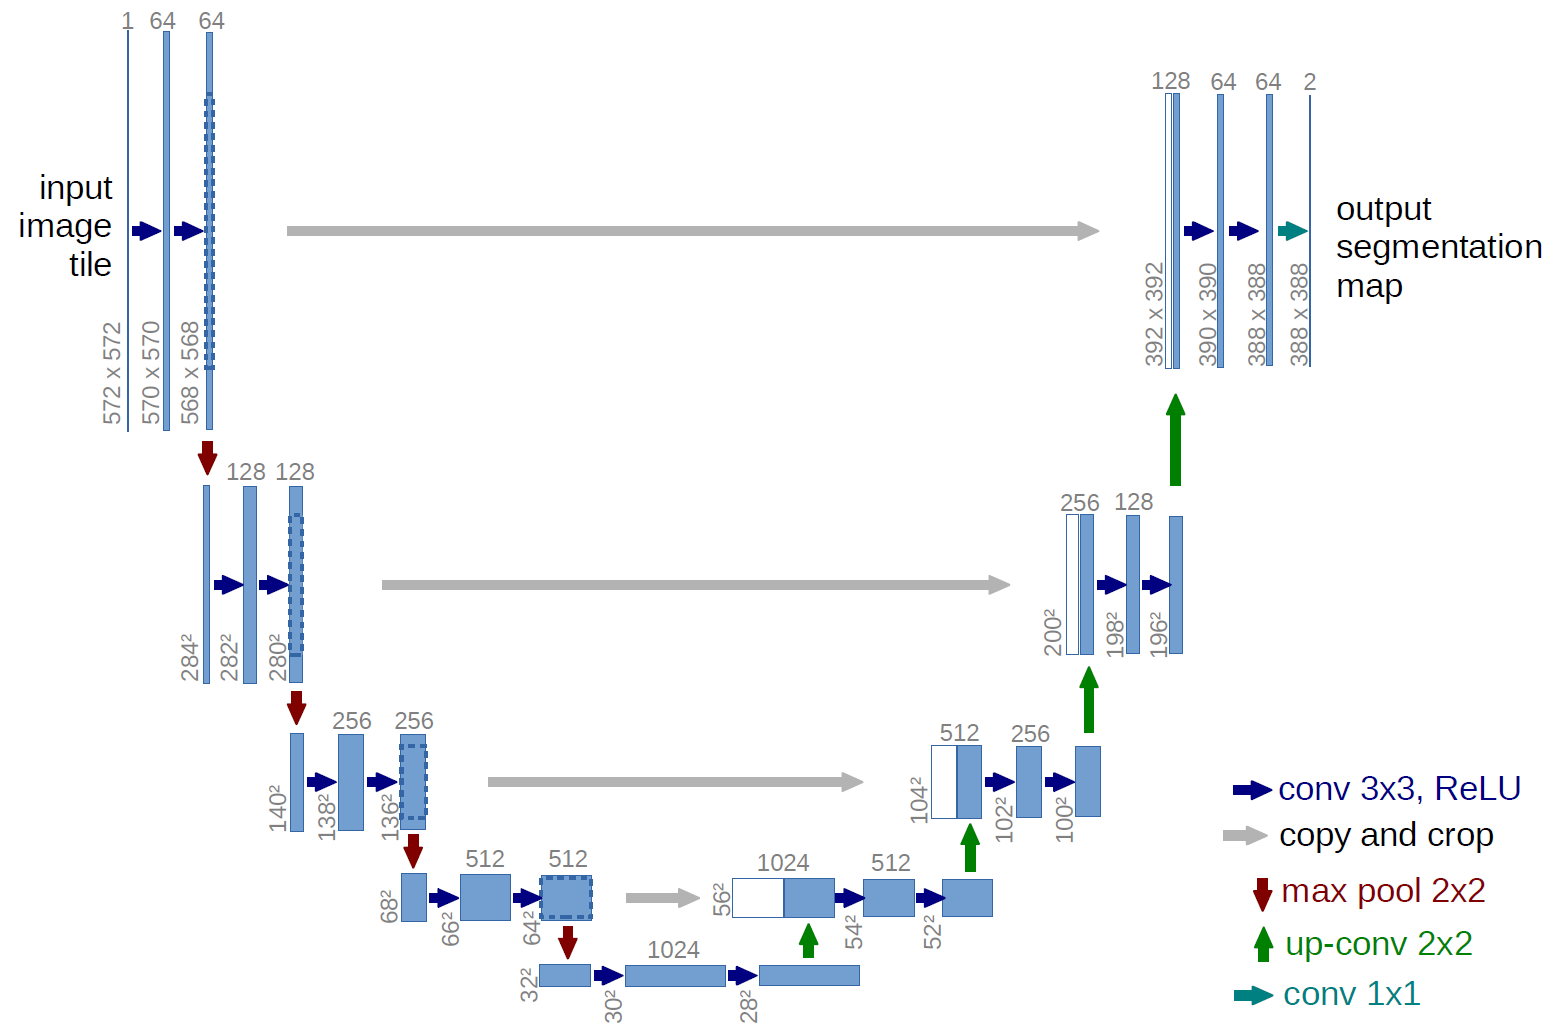
\includegraphics[width=.7\linewidth ]{images/u-net-architecture.png} }}%

\begin{figure}[htp] 
        \centering
        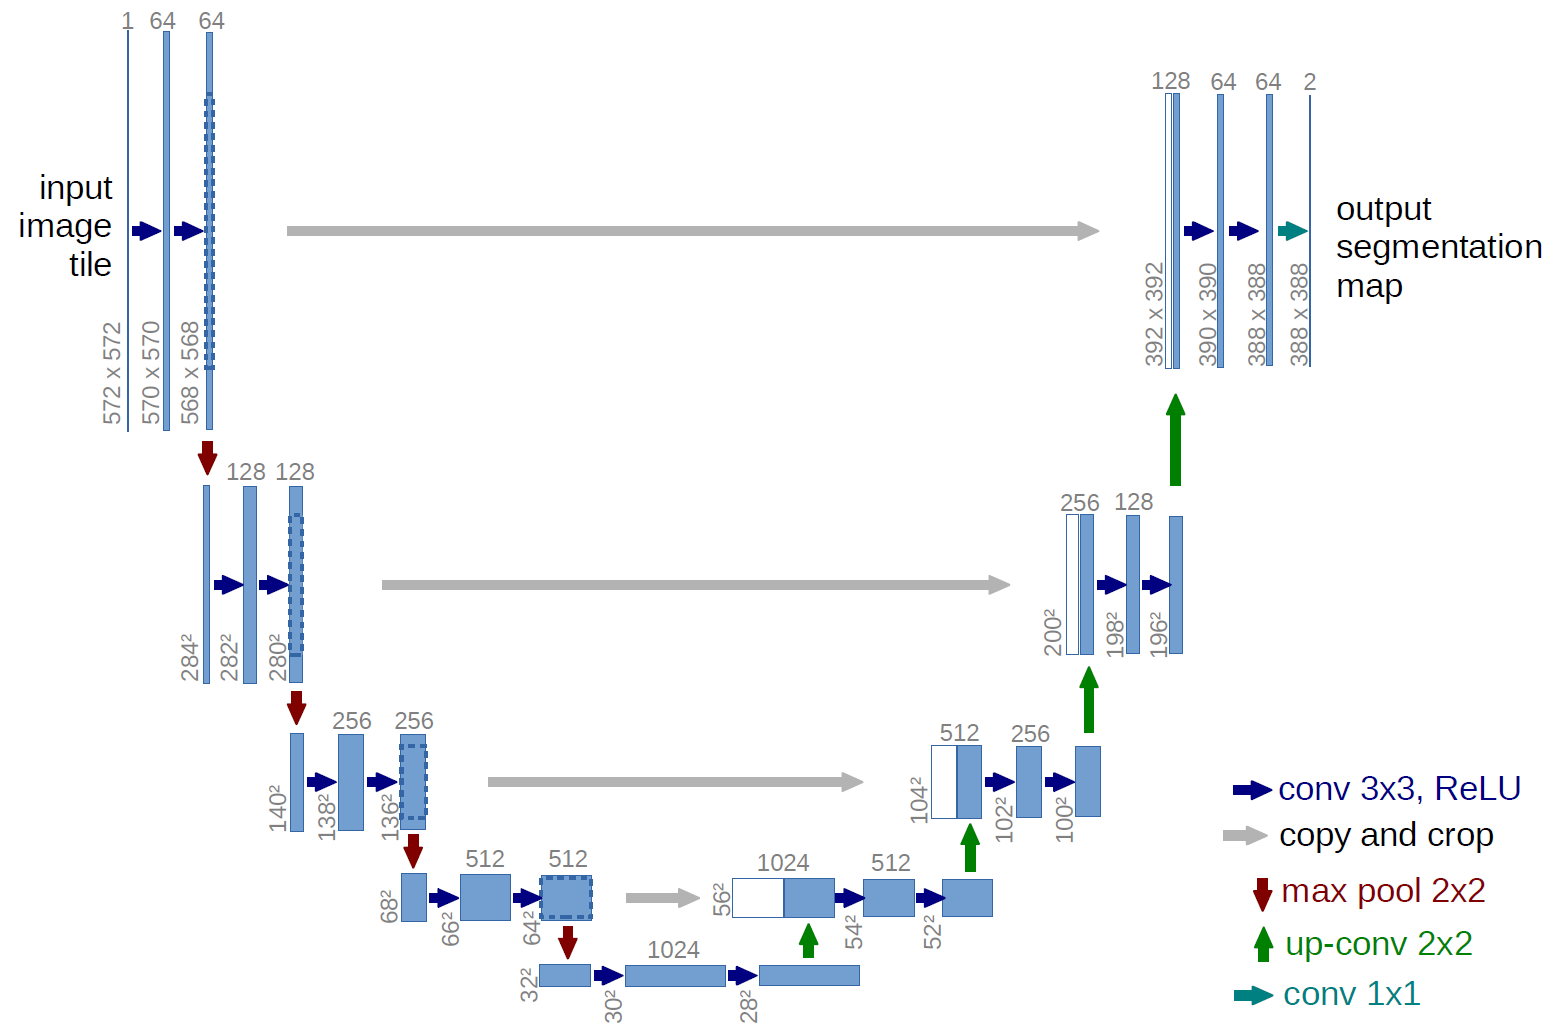
\includegraphics[width=0.8\textwidth]{images/u-net-architecture.png}
        \caption{U-Net Architecture \cite{u-net}}%
        \label{fig:u-net}%
\end{figure}

This architecture was initially designed for biomedical image segmentation and is an improvement on the FCN architecture. \cite{u-net} It has become a popular choice for image segmentation as it requires fewer training images. 
This architecture consists of an encoder and a decoder part and these are connected by a bridge in the bottom-most part of the image. 

\textbf{Encoder Network:} This network extracts features with a sequence of encoder blocks. In the figure above this consists of a 3x3 convolution, then a ReLU activation function and then a max pooling layer. While going down the encoder or the contracting path, the dimensions are halved as compared to the previous layer and the feature channels are doubled. 

\textbf{Skip Connection:} From the activation function of each layer of the encoder network, the output generated is used and concatenated to the corresponding layer of the decoder network. These connections are useful as they retain features that are useful in obtaining better semantic maps.

\textbf{Decoder Network:} In the decoder network, the semantic segmentation mask is generated. A 2x2 upscale convolution is performed. The skip connection is concatenated to each layer of the decoder network. Then two 3x3 convolutions are used and a ReLU activation function follows the skip connection. In this network, the dimensions are doubled while the feature channels are reduced by half. 
The last decoder goes through a 1x1 convolution with sigmoid activation. This function gives the segmentation mask representing the classification.

\textbf{Bridge:} This connects the encoder and decoder part. It has two 3x3 convolutions, and each convolution is followed by a ReLU activation function.

\newpage
\section{Methodology}

\subsection{Steps and deliverables}

The code for this project is available at \href{https://github.com/SimonDeussen/dope-drone-desegmentation-dlrv.git}{\textbf{Deep Learning for segmentation}}
The instructions to run the code is written in the "ReadMe" file of the repository

\vspace{10px}

The adopted methodology involves semantic segmentation of the aerial images of forest using deep learning techniques 
using ensembling of 3 different U-Net architectures with different backbones. The implementation consists of 4 major steps as shown in Figure \ref{fig:steps}. 
1st step consists of loading the training images along with their labelled masks and resize to cope with limited memory of the system.  2nd step is learning a 
good deep model capable of effective pixelwise classification of an image. In in last step trained model is then evaluated for accuracy of detection as well 
as localization of regions belonging to the non-forest areas in the images. 
\begin{figure}[htp] 
        \centering
        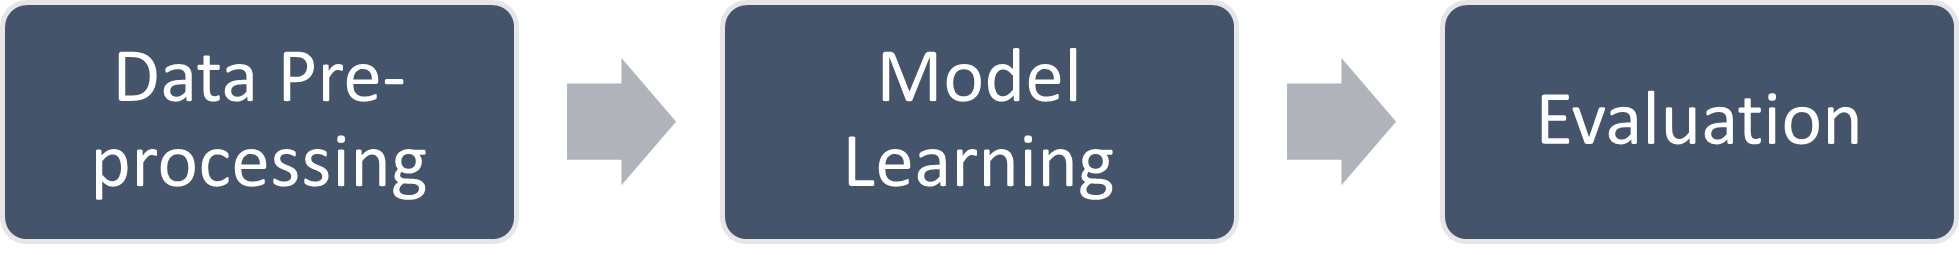
\includegraphics[width=0.8\textwidth]{images/fig3.png}
        \caption{Project steps}%
        \label{fig:steps}%
\end{figure}

\subsection{Data Pre-processing}

The dataset used for model training and evaluation consists of  5108 aerial images of dimensions 256x256. The dataset is obtained from land cover 
classification track in \href{https://www.kaggle.com/balraj98/deepglobe-land-cover-classification-dataset}{\textbf{DeepGlobe Challenge }}
. Each image has been provided with a binary mask image as label for the image the defines region of interest to distinguish between forest and non-forest regions 
in the image.

The size of the data set was increased by creating augmented images of the data set. The resulting data set contained 25,540 images. The following data augmentations 
were done 
\begin{itemize}
        \item Rotation randomly between -180 and 180 degrees
        \item Horizontal flip
        \item Vertical flip
        \item Vertical shift randomly between -64 and 64
        \item Horizontal shift randomly between -64 and 64
\end{itemize}

Each of the above 5 augmentations were performed on all the images and hence the data set was increased five fold

\subsection{Model learning}

\textbf{Model Architecture}
\vspace{20px}


Model trained for solving the problem at hand consists of U-net with 3 different backbones i.e. VGG19, ResNet and InceptionV3. Unet itself is an extended 
implementation of an encoder-decoder topology of  fully convolutional network. The intuition behind Unet is to encode the image through 
a CNN (encoder-downsampling stage) and then decode it back (decoder-upsampling stage) that gives the segmentation mask.  The backbone is the architectural
 element which modifies the layers in the encoder network and hence modifies the feature extraction and encoding approach area and hence it also determines how 
 the decoder network should be built accordingly that compliments the new modified encoder network.
Since each architecture among Vgg, ResNet and Inception excels in different application hence combining all three provides best results in our implementation. 
Figure \ref{fig:U-Net with ResNet} shows a general architecture of U-Net implemented with ResNet backbone. Summary of the three models have been given in appendix

All the models are initialized with pretrained weights on ImageNet which not only reduces the training time but improves the learning capability of model in small dataset. 


\begin{figure}[htp] 
        \centering
        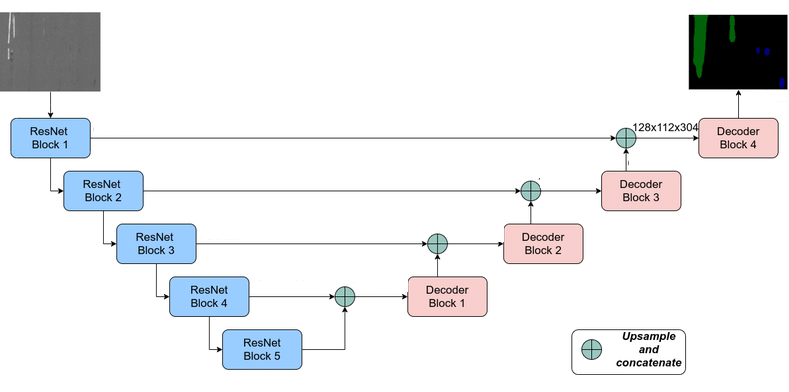
\includegraphics[width=1.2\textwidth]{images/fig4.png}
        \caption{U-Net with ResNet}%
        \label{fig:U-Net with ResNet}%
\end{figure}

\begin{figure}[htp] 
        \centering
        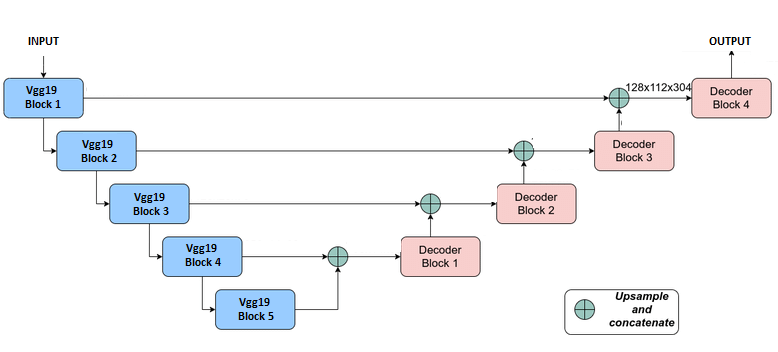
\includegraphics[width=1.2\textwidth]{images/fig7.png}
        \caption{U-Net with VGG19}%
        \label{fig:U-Net with VGG19}%
\end{figure}

\begin{figure}[htp] 
        \centering
        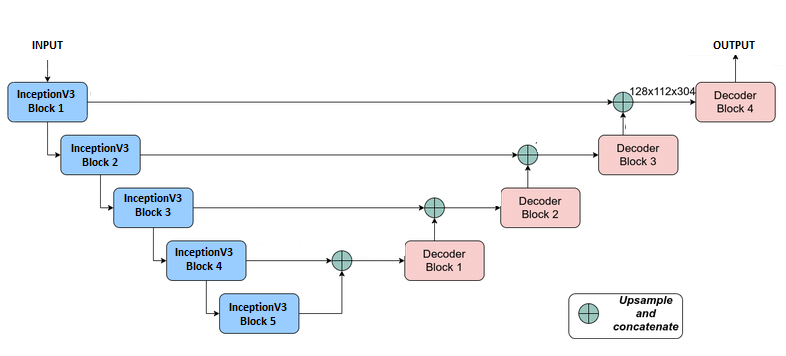
\includegraphics[width=1.2\textwidth]{images/fig8.png}
        \caption{U-Net with InceptionV3}%
        \label{fig:U-Net with InceptionV3}%
\end{figure}


\subsection{Model Training}

Three different U-net architectures with 3 different backbones are individually trained on the same training dataset.  
Table \ref{tab:Training} shows training parameters used during training of  all 3 models.

% Please add the following required packages to your document preamble:
% \usepackage[table,xcdraw]{xcolor}
% If you use beamer only pass "xcolor=table" option, i.e. \documentclass[xcolor=table]{beamer}
\begin{table}[h]
        \centering
        \begin{tabular}{|l|l|}
        \hline
        \textbf{Parameter} & \textbf{Name}              \\ \hline
        Loss function      & Binary focal dice loss     \\ \hline
        Metric 1           & IOU score(threshold =0.5)  \\ \hline
        Metric 2           & F1 score ((threshold =0.5) \\ \hline
        Optimizer          & Adam                       \\ \hline
        Batch Size         & 8                          \\ \hline
        Epochs             & 100                        \\ \hline
        \end{tabular}
        \caption{Training Parameters}
        \label{tab:Training}
        \end{table}



Figure \ref{fig:Training progress model 1}, \ref{fig:Training progress model 2}, \ref{fig:Training progress model 3} show individual training progress of all models of U-Net with different backbones. Figure-9 shows training and validation loss of U-Net model
with ResNet34 backbone on right and IoU during training on left. It can be seen that during learning progress training loss shows a clear minimizing trend 
whereas validation loss shows randomly increasing loss because of poor labelling of ground truth data. IoU also tells the same story where training IoU
follows the loss trend for training data where as IoU factor for validation data does not improves more than 67%.  

\begin{figure}[htp] 
        \centering
        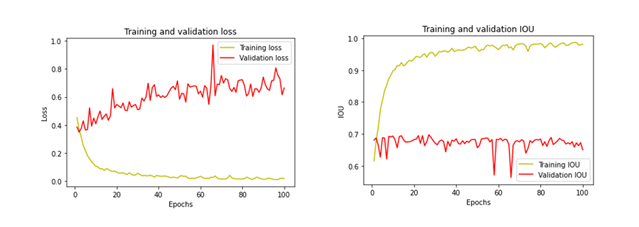
\includegraphics[width=1.2\textwidth]{images/fig9.png}
        \caption{Training progress model 1}%
        \label{fig:Training progress model 1}%
\end{figure}


Figure \ref{fig:Training progress model 2} shows same training validation loss for model-2 as observed for model-1 as well as IoU observed on validation data does not improve more 
than 67\% despite training data IoU reached to almost 99\%

\begin{figure}[htp] 
        \centering
        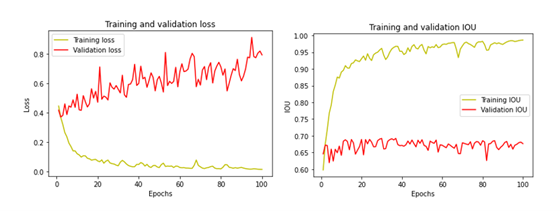
\includegraphics[width=1.2\textwidth]{images/fig10.png}
        \caption{Training progress model 2}%
        \label{fig:Training progress model 2}%
\end{figure}


Figure \ref{fig:Training progress model 3} shows some different trends for both losses and IoU for training and validation data during training of U-Net using Vgg19 backbone.
 The validation loss showed decreasing trend in the beginning unlike previous 2 models. IoU on validation data did not show much variations and mostly 
 stayed constant at around 67\%.  
 \begin{figure}[htp] 
        \centering
        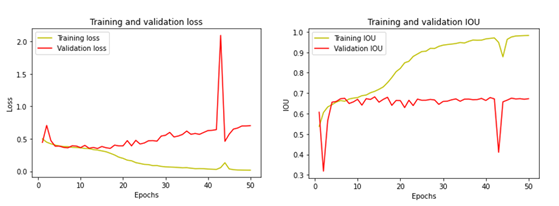
\includegraphics[width=1.2\textwidth]{images/fig11.png}
        \caption{Training progress model 3}%
        \label{fig:Training progress model 3}%
\end{figure}

\textbf{Ensembling of models for semantic segmentation}
\vspace{10px}

All the 3 different variants of U-net are ensembled together to give pixel level classification of each image. 
Following random combination of weights are selected to get the weighted average of final prediction.  
w1 =0.3 ,  w2= 0.5 ,  w3= 0.2
A best combination of weights for each model is selected that gives best result on prediction on individual prediction of each model. 
A combination of weighted average of model gives the final prediction, using equation 1
                    $$P=  w1*p1 + w2*p2 + w3*p3   $$
Where
P= final prediction 
P1 = prediction by model 1 
P2 = prediction by model 2
P3 = prediction by model 3

\subsection{Evaluation strategy}



The presented approach is evaluated for its accuracy of distinguishing forest regions from non-forest regions in the aerial images. The model tested on already separated test from original dataset consists of 500 images. At test time the implemented model produces for given image a binary image with two regions defined as forest and non-forest images. These predicted binary images are then compared with the provided labels to calculate pixel wise results. IoU factor is used for evaluating the predicted region with provided one. 
IoU is measured using following mathematical relation:

$$IOU=\frac{Intersection\;area}{Total\;area }$$
IoU scores can further be converted to mean average precision, but further analysis is not performed due to time constraints. 


\subsection{Results and Discussion}

The ensembling approach presented in above section provided an average pixel classification accuracy of 32\%. This low value of accuracy is due to poor 
labeling of the dataset. Visual inspection of the predicted images has shown better results on average compared to the provided labels and hence despite the 
low accuracy score the trained model gives acceptable results for real application. IoU score calculated over all 
three models and ensemble model are as following:
Following are the mean IoU obtained for each individual model as well as using the ensembled model.
\vspace{10px}

IOU Score for model1 =  0.6515429

\vspace{3px}

IOU Score for model2 =  0.6777154

\vspace{3px}
IOU Score for model3 =  0.67442536

\vspace{3px}

IOU Score for weighted average ensemble =  0.68797314 

\vspace{3px}
Since the provided ground truth data was poorly labelled as can be seen in the (Testing label ) in figure \ref{fig: Prediction with Bad IoU scores} - \ref{fig: Predictions with Good  IoU scores}hence IoU score did not provided got score 
despite the fact visual inspection showed extremely impressive prediction of the forest and non-forest regions as shown in 
Figure \ref{fig: Predictions with Good IoU scores} and \ref{fig: Prediction with Bad IoU scores}

\begin{figure}[htp] 
        \centering
        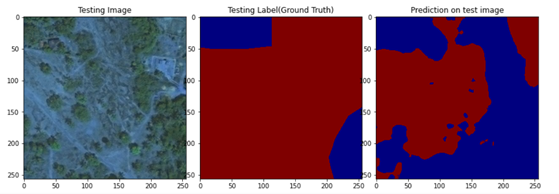
\includegraphics[width=1.2\textwidth]{images/fig12.png}
        \caption{ Prediction with Bad IoU scores}%
        \label{fig: Prediction with Bad IoU scores}%
\end{figure}

\begin{figure}[htp] 
        \centering
        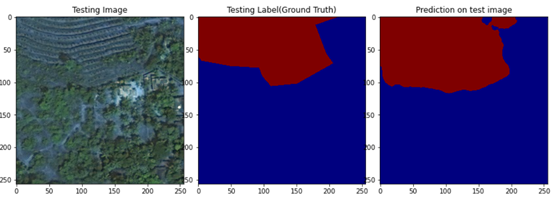
\includegraphics[width=1.2\textwidth]{images/fig13.png}
        \caption{ Predictions with Good  IoU scores}%
        \label{fig: Predictions with Good  IoU scores}%
\end{figure}



The main rule has been played by the weight initialization using ImageNet trained weights. The models with weights trained on ImageNet has already learned the 
notion of learning useful object in the real-world images. Training on aerial images further allowed the model to adapt according to the required image regions. 

Given below are some of the more 

\newpage
\bibliographystyle{ieeetr} % Use the plainnat bibliography style
\bibliography{bibliography.bib} 

\newpage
\section{Appendix}


\textbf{Please see next page}

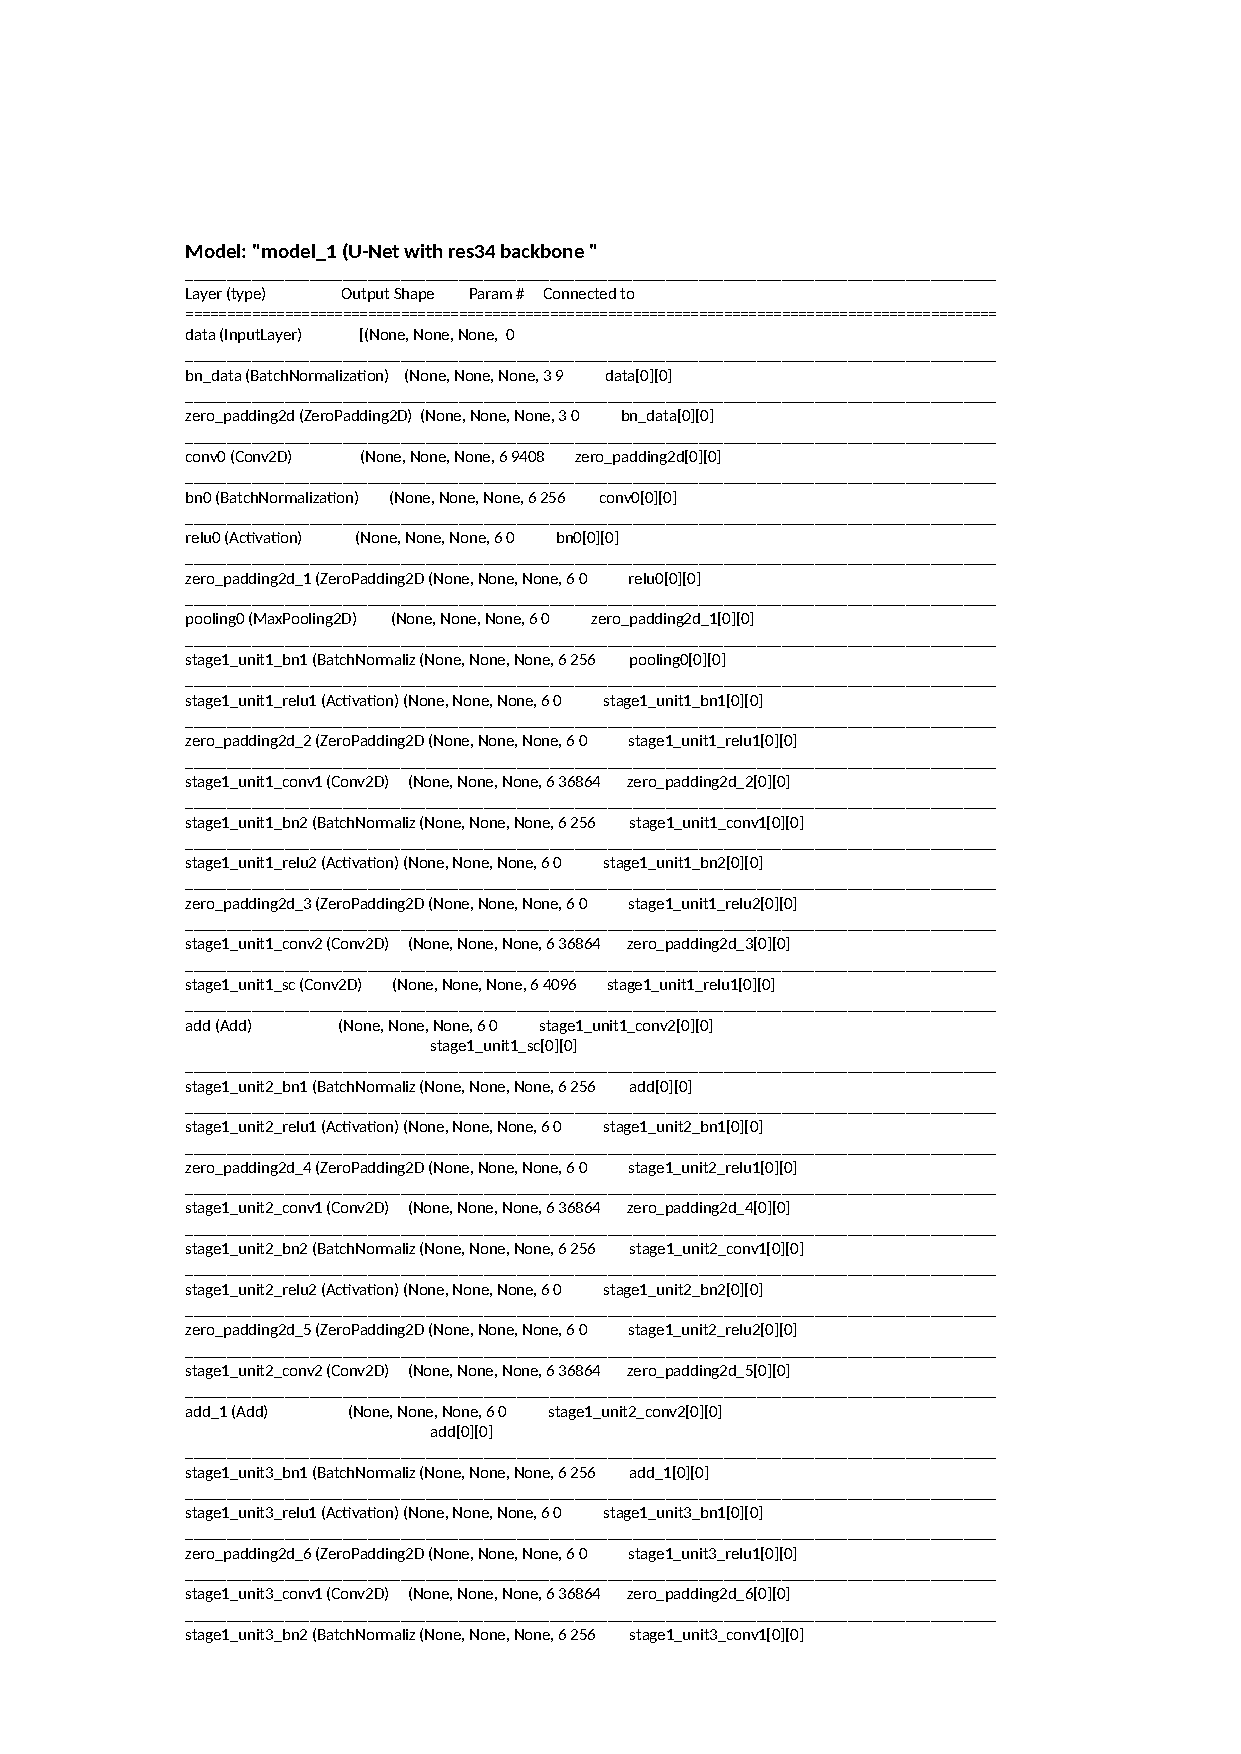
\includepdf[pages=-]{appendix.pdf}

 
\end{document}
